% ACM Computing Surveys source using the official, unmodified acmart class.
\documentclass[manuscript,review,anonymous]{acmart}
\usepackage{tabularx}
\newcolumntype{Y}{>{\raggedright\arraybackslash}X}
\acmJournal{CSUR}
\setcopyright{none}
\settopmatter{printacmref=true,printfolios=true}
\acmDOI{}
\acmYear{2026}
\copyrightyear{2026}

\title{World Models for Physical AI: Learning to Predict, Plan, and Act in the Real World}
\author{Anonymous Author(s)}

\begin{abstract}
World models provide a means of representing how physical environments evolve and how an agent's actions may change them. Their relevance to Physical AI extends across predictive representation learning, simulation, planning, policy training, and execution monitoring. These roles place different demands on what a model predicts, how actions condition its predictions, and how the predictions are used; architecture labels alone do not reveal whether a system supports prediction, decision making, or physical execution. This survey examines world models through these three questions, connecting model-based control with visual and latent prediction, structured physical representations, multimodal interaction data, and robot policies. We organize the discussion into foundations, data and model design, integration with decision making, and evaluation and deployment, and trace each system claim through its prediction target, action interface, operational role, and evaluation setting. Across the mapped evidence, three distinctions recur. First, offline predictive quality, simulated closed-loop performance, and physical closed-loop utility are related but not interchangeable. Second, system-level gains often combine data, representation, policy, planning, and inference changes, so attribution to a world-model component requires matched controls. Third, safety evidence spans conditional guarantees, empirical violation reduction, monitoring, intervention, and recovery rather than a single strength ranking. We also examine reasoning-policy hybrids as an emerging interface between general-purpose reasoning and robot control. The resulting framework connects design choices to evidence appropriate to their role while preserving the scope and denominator of each claim.
\end{abstract}

\begin{CCSXML}
<ccs2012>
 <concept>
  <concept_id>10010147.10010178.10010187.10010192</concept_id>
  <concept_desc>Computing methodologies~Robotics</concept_desc>
  <concept_significance>500</concept_significance>
 </concept>
 <concept>
  <concept_id>10010147.10010257.10010258.10010259</concept_id>
  <concept_desc>Computing methodologies~Reinforcement learning</concept_desc>
  <concept_significance>300</concept_significance>
 </concept>
</ccs2012>
\end{CCSXML}
\ccsdesc[500]{Computing methodologies~Robotics}
\ccsdesc[300]{Computing methodologies~Reinforcement learning}
\keywords{world models, Physical AI, robot learning, predictive representations, vision-language-action models, model-based control}

\begin{document}
\maketitle

\section{Foundations and Scope}
\label{sec:foundations}

\subsection{Introduction}
Physical AI concerns agents whose decisions change a physical environment. For a robot, choosing an action requires more than identifying a goal: the system must also contend with what is currently observable, how its body can move, and how objects may respond. A world model makes some of these consequences available as predictions. The central question for this survey is how such predictions contribute to learning and acting under the constraints of physical interaction.

Predictive models can support control through different computational routes. In \emph{World Models}, learned visual and temporal representations support policy learning, including training inside a learned environment~\cite{ha2018worldmodels}. PlaNet instead learns latent dynamics from images and uses online planning to select actions~\cite{hafner2019planet}. These examples motivate a distinction between using prediction to construct a policy and querying predictions while choosing an action. Their experimental settings establish particular uses of learned dynamics rather than a general guarantee of real-world competence.

Robot policies offer a complementary interface: they map observations and instructions to actions. OpenVLA, for example, adapts a vision-language backbone using robot demonstrations to produce visuomotor behavior~\cite{kim2024openvla}. This interface does not by itself expose a future-state predictor that can be queried under alternative actions. The distinction is functional: a policy may contain useful knowledge of dynamics, while an explicit prediction interface provides an additional object that can be inspected, optimized against, or compared with subsequent observations.

The relationship between representation learning and action-conditioned prediction also deserves separate treatment. V-JEPA~2 combines action-free video pretraining with a subsequent action-conditioned model, V-JEPA~2-AC, for robotic planning~\cite{assran2025vjepa2}. The stages serve different purposes and should not be assigned the same control interpretation solely because they share a representation. This motivates recording both the supervision that creates a representation and the interface through which a controller later uses it.

We organize the survey around three questions: \emph{what is predicted, how actions enter the model, and where prediction is used}. These are the survey's comparison axes. Together they connect data and model design to operational roles without requiring all systems to share one architecture or output space. A video generator, a latent predictor, and a structured dynamics model may address different parts of this design space; their comparison should identify the relevant state variables, time horizon, and control interface before assessing performance.

The same role-based approach guides evaluation. Evidence that a model predicts observations accurately supports a different claim from evidence that its predictions improve action selection. Likewise, a closed-loop task result must be interpreted with its task distribution, controller, inference budget, and failure conditions. Our synthesis therefore records predictive performance, downstream use, and deployment conditions separately. This is an analytical choice of the survey, not a universal ranking of papers or a requirement that every supporting component demonstrate a complete robot system.

The article follows four parts. Section~\ref{sec:foundations} establishes the scope and comparison axes. Section~\ref{sec:data} examines the data, representations, and modeling choices that determine which consequences can be learned. Section~\ref{sec:policy} studies how prediction interacts with policies, planning, memory, and recovery. Section~\ref{sec:evaluation} organizes evaluation, reliability, safety, and open problems around the claims that a deployed system must substantiate. A companion literature catalog retains the seven collection categories used by the project and links them to the writing process.

\subsection{Working Definitions and Inclusion Boundaries}
We use \emph{world model} for a learned model that predicts aspects of an environment's evolution from available information. For an action-conditioned world model, the inputs additionally specify actions or other interventions. The predicted variables may be observations, latent states, object relations, physical quantities, or task-relevant consequences. This working definition accommodates models learned from passive observations as well as interaction data; it does not assume that every predictive representation already provides an executable robot-action interface.

For analysis, let a history summarize the agent's observations and past actions. A policy maps this information and a goal to an action or action sequence. An action-conditioned world model maps the history and a proposed action sequence to predicted consequences. A controller turns the selected command into realized motion. Separating these interfaces lets us ask whether a failure originates in prediction, action selection, or execution, even when some interfaces are implemented inside a shared network.

The literature corpus includes both direct methods and supporting work. Learned simulators, predictive models used for planning, and prediction-guided policy learning provide direct cases. Datasets, analytical simulators, representation encoders, sensors, and policy baselines provide supporting context according to their demonstrated roles. Their inclusion does not imply that each item is itself a learned world model. In particular, the presence of a reasoning model in a control loop is insufficient to identify an explicit future-prediction mechanism.

\begin{figure}[t]
  \centering
  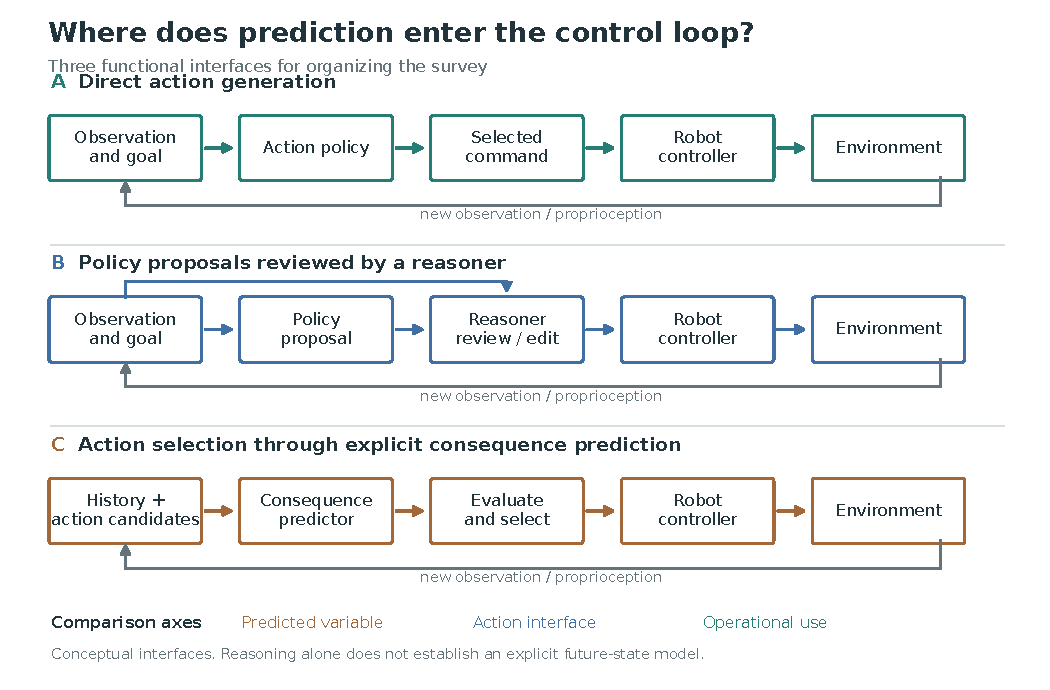
\includegraphics[width=\linewidth]{figures/fig01_prediction_policy_interfaces.pdf}
  \caption{Interfaces linking observation to physical action. The schematic distinguishes direct action generation, policy proposals reviewed by a reasoning model, and candidate actions evaluated through an explicit consequence predictor. Arrows denote interface-level information flow, not the internal architecture of any one model. Observation feedback closes each loop.}
  \Description{Three horizontal control loops. The first maps observations through a policy and controller to the environment. The second inserts a reasoner that reviews policy proposals and also receives observations. The third predicts consequences of action candidates before evaluation, selection, and control. Each loop returns new observations from the environment.}
  \label{fig:interfaces}
\end{figure}

\section{Data, Representations, and Predictive Models}
\label{sec:data}

\subsection{Organizing Data by Available Supervision}
We organize data sources by the supervision they provide for prediction and action. Passive observations support learning regularities of appearance and temporal evolution. Interaction records additionally associate an agent's commands with subsequent observations. The distinction is illustrated by the separate action-free and action-conditioned stages in V-JEPA~2~\cite{assran2025vjepa2}. For each dataset considered in the full review, the comparison will record which actions, timestamps, state measurements, and outcomes are available, and whether the data include failures or only successful demonstrations.

\subsection{Comparing Representations by Their Use}
The relevant prediction space depends on how a downstream system consumes the output. PlaNet illustrates planning within a learned latent dynamics model~\cite{hafner2019planet}; a system that generates observations for inspection exposes a different interface. Our model comparison will therefore connect each representation to a predicted variable, temporal horizon, action encoding, and use in learning or decision making. Model size and visual quality are retained as attributes rather than treated as substitutes for this functional description.

The collection categories for visual prediction, latent representations, and structured physical or multimodal models provide the literature inputs to this comparison. They are not assumed to form disjoint mathematical classes: a system may use more than one representation, and its placement in the review should explain the role of each component.

\section{Integration with Robot Policies}
\label{sec:policy}

\subsection{Reasoning-Policy Hybrids: The Astra Case}
Recent Astra evaluations motivate distinguishing direct numerical action generation from a hybrid interface that reviews a learned policy's proposals. In Su et al.'s technical report~\cite{su2026astra}, Astra can correct actions proposed by $\pi_{0.5}$. On ten selected RoboDojo tasks with five aligned cases per task, the authors report 48\% success for the hybrid and 26\% for direct Astra control. The public-policy comparisons use published reference scores rather than same-seed reruns. These findings support a bounded discussion of complementary action-generation and correction roles; they do not isolate a future-prediction mechanism.

A separate evaluation by Zhang et al.~\cite{zhang2026unexpected} covers all 42 RoboDojo tasks, with 50 episodes per task for Astra. It reports 22.48\% average success over 2,100 trials and a capability profile that varies substantially across task types. This broader result should be discussed alongside the selected-task hybrid study, while keeping their task sets and denominators separate.

The Galbot team's September 29 preprint~\cite{galbot2026astra} extends the investigation across six domains, including cooperation with learned policies. Its gripper-manipulation discussion includes the same 48\% RoboDojo hybrid result. We treat the overlapping result as part of one evidence series rather than a second independent replication. The paper also documents inference constraints, including paused physics during its locomotion reasoning calls. This makes the relation between simulated success and time-critical control an explicit part of the discussion.

Black Forest Labs' FLUX~3 Action report~\cite{bfl2026flux3action} examines another combination: a fast action policy supplies proposals that Astra may accept, edit, replace, or stop. The report connects hybrid performance to inference cost and elapsed time, alongside task completion. This provides an industrial case for evaluating the entire decision loop, with the report's own protocol and provenance retained.

For world-model research, these interfaces raise a specific attribution question. Does a hybrid improve because it predicts action consequences, identifies the correct target, repairs a proposal, or uses more computation? A useful comparison would hold the base policy, observations, control limits, and inference budget fixed while varying the information supplied to the reviewer: current observations, proposed actions, and explicit predicted consequences. This comparison is a proposed evaluation design of the survey, not an experiment established by the cited reports. It connects the Astra discussion to the article's main question: when, and through which interface, does prediction change action selection?

\begin{table}[t]
\caption{Interfaces and study scope in the Astra discussion. This is a provenance table, not a cross-paper performance leaderboard.}
\label{tab:astra}
\small
\begin{tabularx}{\linewidth}{@{}p{.19\linewidth}YY@{}}
\toprule
Source & Interface examined & Scope retained in the comparison \\
\midrule
Su et al.~\cite{su2026astra} & Direct action generation; review of $\pi_{0.5}$ proposals & Selected tasks and aligned cases; public policy scores are reference results. \\
\addlinespace
Zhang et al.~\cite{zhang2026unexpected} & LLM as policy & Full 42-task RoboDojo evaluation for Astra. \\
\addlinespace
Galbot Team~\cite{galbot2026astra} & Direct and hybrid interfaces across domains & Domain-specific protocols; overlap with the earlier report. \\
\addlinespace
Black Forest Labs~\cite{bfl2026flux3action} & FLUX~3 Action proposals with Astra review & Report-specific hybrid protocol and resource accounting. \\
\bottomrule
\end{tabularx}
\end{table}

\section{Evaluation, Reliability, and Research Directions}
\label{sec:evaluation}

\subsection{Match Evidence to the Operational Claim}
We distinguish three questions in evaluating a world-model-based system. First, does the predictor represent the variables relevant to its stated role? Second, do its outputs affect the downstream decision in the intended way? Third, does the complete system operate under the timing and environmental conditions of the claimed application? These questions define the structure of the evaluation discussion; they are not a single score or a ladder that every supporting dataset or component must climb.

The Astra studies provide a useful case for this separation. A reported task outcome concerns an implemented control interface and a particular evaluation protocol. Establishing that an explicit world model caused an improvement requires an additional comparison that isolates the prediction component. Similarly, results collected with paused simulation do not test the consequences of reasoning delay in a continuously evolving environment. These distinctions determine which conclusions can be transferred from the reported experiment to a deployment setting.

\subsection{Reliability as a System Property}
For each operational role, the review will connect potential failures to observable checks and available responses. A planner may select actions whose predicted consequences are inaccurate; a monitor may fail to detect divergence; a controller may fail to realize a selected command. The corresponding analysis should identify what is measured, how a discrepancy changes execution, and whether the response itself has been evaluated. This organization keeps safety claims attached to the behavior of the complete system.

The next synthesis step is to populate these comparisons with verified studies of uncertainty, distribution shift, failure recovery, and runtime constraints. The current draft establishes the comparison structure. It does not yet claim comprehensive coverage of these topics or a completed systematic-review screening process.


\bibliographystyle{ACM-Reference-Format}
\bibliography{references}
\end{document}
